\documentclass[11pt]{article}

\usepackage[margin=1.0in]{geometry}
\usepackage[usenames,dvipsnames]{color}
\usepackage{lmodern}
\usepackage[T1]{fontenc}
\usepackage{amsmath}
\usepackage{array}
\usepackage{bigstrut}
\usepackage{booktabs}
\usepackage{enumerate}
\usepackage{fancyvrb}
\usepackage{framed}
\usepackage{graphicx}
\usepackage{hyperref}
\usepackage{ifthen,version}
\usepackage{longtable}
\usepackage{textcomp}
\usepackage{todonotes}
\usepackage{wrapfig}
\usepackage{subcaption}
\usepackage{mwe}
\hypersetup{
    colorlinks,
    %pdfborderstyle={/S/U/W 1}
    linkcolor={red!50!black},
    citecolor={blue!50!black},
    urlcolor={blue!80!black},
}
\usepackage{caption}
\usepackage{subcaption}

\setlength\bigstrutjot{3pt}

\newcolumntype{L}[1]{>{\raggedright\let\newline\\\arraybackslash\hspace{0pt}}m{#1}}

\setlength{\parindent}{0pt}
\setlength{\parskip}{5pt}
\newcommand{\la}{\textlangle{}}
\newcommand{\ra}{\textrangle{}}
\newcommand{\wtodo}[1]{\todo[author=WT,inline]{#1}}

\begin{document}
\title{RPAL ROS \& Programming Skills Assessment}
\date{}
\author{}

\maketitle

\section{Objective:} 

Demonstrate understanding of basic ROS usage and Python (or C++) programming, as well as some basic
robotics concepts. This project will be used to assess your readiness to begin working in RPAL as an
undergraduate researcher.

\section{Collaboration Policy:} 

This assignment \textbf{must be completed alone}. You are permitted to use any internet resources
(short of asking for help on a forum, etc.), books, tools, what have you, but you may \textbf{not}
collaborate with anyone and you may \textbf{not} ask any grad students or anyone else for
assistance. This is an assessment of you and your current skills; if you violate this policy we
cannot make an accurate assessment and will not be able to work with you.

Note that you can come to us if you are truly stuck. If the issue is a bug or simple
misunderstanding with the provided code, we can help you out and you can get back to the assessment.
\textbf{However}, if you come to us and the provided code is working correctly (i.e.\ the error is
with your code), that will constitute termination of the project and we will assess your work in
whatever state it is in.

\section{Running the simulator framework}

We have provided a simulation framework for you to develop and test your code. In order to use the
framework, you'll need to carefully follow these instructions.

\subsection{Setup}

Do these steps \emph{once}, before starting your work. We also recommend using Git to store your
partial progress. Note that successfully completing the setup process is part of the assessment.

\subsubsection{ROS}

Follow the instructions here: \url{https://wiki.ros.org/melodic/Installation} to install ROS
Melodic.

\subsubsection{V-REP}

The simulation framework is based around
\href{http://www.coppeliarobotics.com/downloads.html}{V-REP}, which you can download at that link.
Get the ``Pro EDU'' version for Linux and extract the files to some directory
(\texttt{\textasciitilde/V-REP} is a good choice). Finally, copy the file
\texttt{libv\_repExtRosInterface.so} from this directory to wherever you extracted V-REP.

\subsubsection{Catkin Workspace}

Before starting the project, you need to set up a catkin workspace. To do this, follow the
instructions here: \url{https://wiki.ros.org/catkin/Tutorials/create_a_workspace}. Afterwards, copy
the \texttt{src} subdirectory from this package into \texttt{<YOUR CATKIN ROOT>/src/rpal\_ros\_test}
and run \texttt{catkin build} to build the initial workspace.

\subsection{Using V-REP}

The second part of this assignment will require you to run V-REP. To this end, we have provided a
V-REP scene file, \texttt{assessment.ttt}, in this directory. Use the following steps to run the
simulator:
\begin{enumerate}
  \item Start \texttt{roscore}.
  \item (assuming you extracted V-REP to \texttt{\textasciitilde/V-REP}), run
  \texttt{\textasciitilde/V-REP/vrep.sh assessment.ttt} in this directory.
  \item Press the "Play" button in the upper toolbar.
  \item Run the commands you need for the particular problem.
  \item Run the commands to execute your code.
\end{enumerate}  

\textbf{To start the simulation, you must hit the play button.}

\section{Assignment:}

RPAL primarily uses ROS and Python for research coding. Thus, you will need to write Python code
using \href{http://wiki.ros.org/rospy}{rospy} to be an effective researcher in the lab. If you need
a refresher for Python, we suggest \href{https://learnxinyminutes.com/docs/python/}{this quick
reference}\footnote{Note that we use Python 3 in most research.}. You should also use the
\href{http://www.numpy.org/}{numpy library} for
\href{https://docs.scipy.org/doc/numpy-1.14.0/reference/generated/numpy.matrix.html}{matrix}
calculations and linear algebra, which is common in robotics research.

If you need a reference for ROS, we suggest the \href{http://wiki.ros.org/ROS/StartGuide}{ROS
``Getting Started'' guide}, the \href{http://wiki.ros.org/rospy}{rospy documentation}, and Jason
O'Kane's \href{https://cse.sc.edu/~jokane/agitr/agitr-letter.pdf}{``A Gentle Introduction to
ROS''}\footnote{Note that AGITR uses C++ instead of Python. The concepts will be the same, but the
language used is different.}.

Implement code to solve the following problems, using the provided simulator framework. Please also
document any difficulties you encountered and how you overcame them in a file named
\texttt{problems.txt}, which you should include with the final submission. When you're done, bundle
up the \emph{whole} \texttt{rpal\_ros\_test} directory into a \texttt{.tar.gz} and send it to us for
assessment.

\section{Part 1: Basic ROS}

This section is intended to assess your knowledge of and ability to use basic ROS concepts.

\subsection{Publishing and Subscribing}
\label{p:topics}

The goal of this problem is to have you learn how to move a turtle using Twist messages and
calculate the distance between turtle and a point.

The work for this problem should be done in file \texttt{pubsub.py}.

\begin{enumerate}[(a)]
  \item In \texttt{\_\_init\_\_}:
    \begin{enumerate}[i.]
      \item First, have your turtle subscribe to \texttt{turtle1/pose} with the callback function
        \texttt{self.update\_pose}. %(\textit{X points})
      \item Have your turtle publish to \texttt{turtle1/cmd\_vel}. %(\textit{X points})
      \item Specify a publishing rate of $10$.
    \end{enumerate}
  \item In \texttt{move}:
    \begin{enumerate}[i.]
      \item Create a Twist message with values that change both the angular and linear velocities
        such that the turtle moves both angularly and linearly.
      \item Publish the Twist message to the velocity publisher.
    \end{enumerate}
  \item In \texttt{update\_pose}:
    \begin{enumerate}[i.]
      \item Set the instance variable \texttt{self.pose} to the information provided by the subscriber.
    \end{enumerate}
  \item In \texttt{calculate\_distance}:
    \begin{enumerate}[i.]
      \item Using \texttt{numpy}, set \texttt{vector} to be the difference between the coordinates
        of the turtle's current pose and the point $(x,y)$. (Hint: Use a \texttt{numpy} array for
        your vector)
      \item Using \texttt{numpy} and \texttt{vector}, set \texttt{distance} to the distance between the
        turtle and the point $(x,y)$.
      \item Set the ROS parameter to \texttt{distance}. (Note: the value of distance must be cast
        to a float).
    \end{enumerate}
  \item In \texttt{pubsub.launch}:
    \begin{enumerate}[i.]
      \item Review the format of this file and understand what it does (see ROS launch file
        documentation for more information).
    \end{enumerate}
\end{enumerate}


\subsection{Single Flower}\label{p:single}

This problem is designed to have you create a node and generate specific behavior for your turtle
using \texttt{numpy} commands. Your turtle's objective is to create a single flower pattern. See
Figure~\ref{fig:1} for exactly what the flower should look like.

The work for this problem should be done in file \texttt{singleflower.py}. Look for the comments
throughout the code that correspond to the instructions in the writeup.

\begin{enumerate}[(a)]
  \item In \texttt{\_\_init\_\_}:
    \begin{enumerate}[i.]
      \item Start a new node with the name `flower'.
      \item Create a publisher that publishes to    \texttt{/turtle1/cmd\_vel} with type
        \texttt{Twist} and a queue size of $10$.
      \item Set your rate to $5$.
    \end{enumerate}
  \item In \texttt{draw\_flower}:
    \begin{enumerate}[i.]
      \item To calculate constants, use \texttt{numpy} to perform the following operations on the
        following matrices:

        $$M_1 = \begin{bmatrix} 
          1.5 & -1.5 & 0\\
          -1.5 & 0 & 2 \\
          2.5 & 0 & 0
        \end{bmatrix} 
        M_2 = \begin{bmatrix} 
          3 & 5 & 9\\
          -1 & 2 & 6 \\
          -3 & 2 & 0
        \end{bmatrix}$$
        $$a = (M_1*M_2)_{(0,1)}+ (M_1*M_2)_{(1,1)}$$
        $$b = -(\langle M_1, M_2 \rangle_{(0,2)} + \langle M_1, M_2 \rangle_{(1,2)}) -1$$
        $$A = \langle M_1, M_2 \rangle_{(0,1)} - \langle M_1, M_2 \rangle_{(0,0)} + 0.5$$
        $$B = -((M_2*M_1)_{(1,2)}-(M_2*M_1)_{(2,1)})$$
        $$\texttt{max\_times} = (\texttt{det}(M_2)/-9) - 4$$
        \textbf{Note}: Angle brackets indicate taking an inner product, subscripts indicate the
        indices of the term that should be taken from a matrix
      \item Each of the above computed constants should be set as rosparams \texttt{a}, \texttt{b},
        \texttt{A}, \texttt{B}, and \texttt{max\_times} with the type \texttt{float}.
      \item In \texttt{while not rospy.is\_shutdown()} section: Use \texttt{numpy} to set angular z
        to $B * \cos(b*count)$ and linear x to $A * \sin(a*count)$. Be sure to publish your velocity
        message and sleep your turtle for your preset rate.
      \item Also in \texttt{while not rospy.is\_shutdown()} section: If value $count$ is greater
        than $2*(\texttt{times})*\pi$:  publish a velocity message with angular $z=5$ and linear
        $x=0$, then increment \texttt{times} by 1 and if \texttt{times} is greater than
        \texttt{max\_times} stop drawing the flower.
    \end{enumerate}

  \item 
    In \texttt{if \_\_name\_\_ == `\_\_main\_\_'} section:

    Create your turtle and have the turtle use your written function to draw a flower. Your final
    product should look something like Figure~\ref{fig:1}.

    \begin{figure}[h]
      \centering
      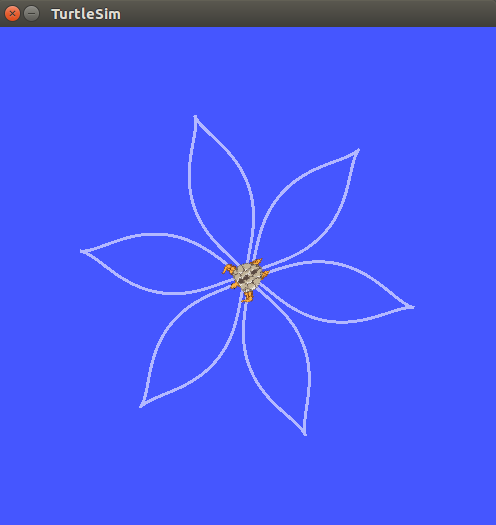
\includegraphics[width=150pt]{figures/p1/problem2.png}
      \caption{For Problem~\ref{p:single}. Single Flower}\label{fig:1}
    \end{figure}  
    %WOW omg replace this image with something more legit before release
  \item In \texttt{singleflower.launch}:
    \begin{enumerate}[i.]
      \item Launch the turtlesim node.
      \item Launch the \texttt{flower\_turtle} node from \texttt{singleflower.py}.
    \end{enumerate}
\end{enumerate}

%%% Local Variables:
%%% mode: latex
%%% TeX-master: "../assessment"
%%% End:

\subsection{Service Clients}\label{p:client}

This problem is designed to introduce the client-service structure. For this question you will be
using our implemented service and writing your own client to create a slightly different single
flower then before. See Figure~\ref{fig:2} for what the flower should look like.

The work for this problem should be done in file \texttt{client.py}.

\begin{figure}[h]
  \centering
  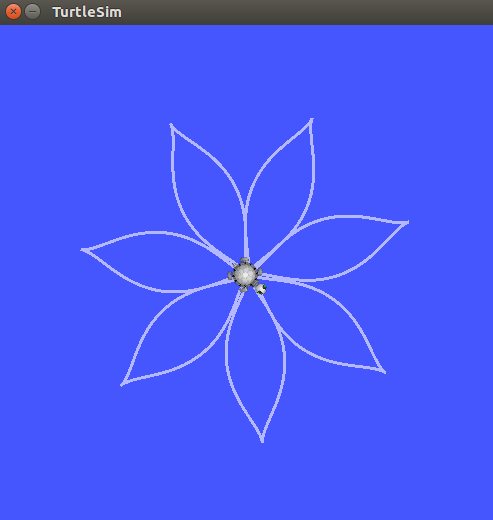
\includegraphics[width=150pt]{figures/p1/problem3.png}
  \caption{For Problem~\ref{p:client}. Service Clients}
  \label{fig:2}
\end{figure}

In \texttt{draw\_flower}:
\begin{enumerate}[(a)]
  \item Initialize your node with the name \texttt{drawing\_turtle}.
  \item Wait for the service \texttt{draw}.

  \item Get a service handle for the draw service. Check \texttt{srv/Draw.srv} and \texttt{rospy}
    documentation for more information.

  \item Make a publisher that publishes to \texttt{/turtle1/cmd\_vel} with type \texttt{Twist} and
    queue size of 10
  \item Make a 5Hz \texttt{Rate}.

  \item Loop, and:
    \begin{enumerate}[i.]
      \item Use the draw service to get the velocity message to publish. Look at \texttt{srv/Draw.srv}
        to determine the parameters and appropriate return name.
      \item Sleep for the previously created rate.
    \end{enumerate}
\end{enumerate}

In the main script:
\begin{enumerate}[(a)]
  \item Call your function to draw the flower!
\end{enumerate}

In \texttt{client.launch}:
\begin{enumerate}[(a)]
  \item Launch the turtlesim node.
  \item Launch the \texttt{draw\_service} node.
  \item  Launch the \texttt{draw\_flower} node.
\end{enumerate}

\subsection{Services}

This problem is meant to have you write a service for the client-service structure. %See \ref{fig:3} for what the flower should look like. The second part has you spawning multiple turtles who will draw flowers. Note that the number of turtles spawned will be between 2 and 5, and their starting locations are randomized (see \texttt{launcher.py} for more details. For an example output see \ref{fig:4}

\subsubsection{Creating a Service}\label{p:service1}

The work for this problem should be done in the file \texttt{draw\_server.py}.

\begin{figure}[h]
  \centering
  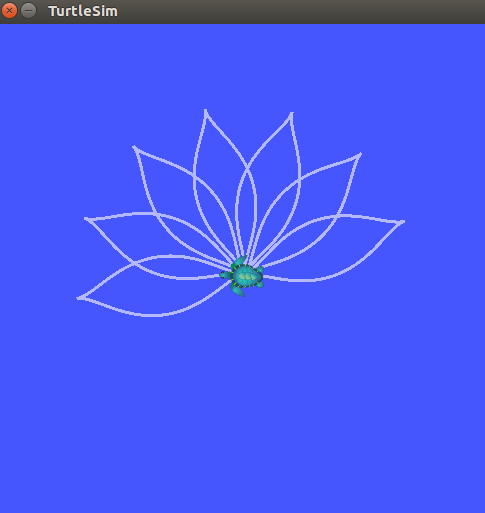
\includegraphics[width=150pt]{figures/p1/problem4a.png}
  \caption{For Problem \ref{p:service1}}
  \label{fig:3}
\end{figure}

\begin{enumerate}[(a)]
  \item In \texttt{draw}:
  \begin{enumerate}[i.]
    \item Initialize \texttt{vel\_msg}.
    \item Set $k$ to be the count parameter of \texttt{req}. %maybe this is too much hand holding idk
    \item To calculate constants, use \texttt{numpy} to perform the following operations on the
    following matrices:

    $$M_3 = \begin{bmatrix} 
      1 & 1 & 2\\
      3 & 5 & 8 \\
      13 & 21 & 34
    \end{bmatrix} 
    M_4 = \begin{bmatrix} 
      1 & 8 & 7\\
      2 & 5 & 3 \\
      9 & 2 & 6
    \end{bmatrix}$$
    
    $$a = det(M_3) -1$$
    
    $$b = -((M_3*M_4)_{(2,0)}-(M_3*M_4)_{(2,2)}) +1$$
    
    $$A = (\langle M_3, M_4 \rangle^T_{(0,0)} - \langle M_3,M_4 \rangle^T_{(1,0)})/10$$
    
    $$B = ((M_3*M_4)^T_{(2,1)}-\langle M_3,M_4 \rangle^T_{(2,1)})/2.0 $$
    
    \item Each of the above computed constants should be set as rosparams \texttt{a}, \texttt{b},
    \texttt{A}, and \texttt{B} with the type \texttt{float}.

  \end{enumerate}

  \item In \texttt{if req.rotate} section:
  \begin{enumerate}[i.]
    \item If \texttt{req.rotate}, set angular z to -3 and linear x to 0.
    \item Otherwise use \texttt{numpy} to set angular z to $B*cos(b*count)$ and linear x to $A*sin(a*count)$.
  \end{enumerate}

  \item Also be sure to return your velocity message before the end of the \texttt{draw} function.
  \item In \texttt{draw\_server}: Create a service with the name \texttt{`draw'}, service\_class
  \texttt{Draw} and handler \texttt{draw}. Please see rospy documentation for further details.
  \item In \texttt{\_\_name\_\_ == `\_\_main\_\_'}: Call your function!
  \item In \texttt{draw\_server.launch}:
  \begin{enumerate}[i.]
    \item Launch the turtlesim node.
    \item Launch \texttt{draw\_service} node from \texttt{draw\_server.py}.
    \item  Launch \texttt{draw\_flower} node from \texttt{client.py}.
  \end{enumerate}

\end{enumerate}
Your resulting flower should resemble Figure~\ref{fig:3}.

\subsubsection{Integrating the pieces}\label{p:service2}

The work for this problem should be done in file \texttt{spawn\_flower.py}. 

\begin{figure}[h]
  \centering
  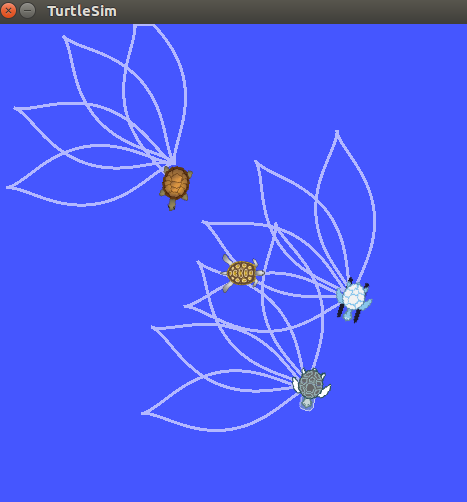
\includegraphics[width=150pt]{figures/p1/problem4b_3turts.png}
  \caption{For Problem~\ref{p:service2}}\label{fig:4}
\end{figure}

\begin{enumerate}[(a)]
  \item In \texttt{draw\_flower}:
  \begin{enumerate}[i.]
    \item Initialize your \texttt{`draw\_turtle'} node
    .
    \item Block while waiting for the \texttt{`spawn'} service to become available. See rospy
    documentation for more information.

    \item In first \texttt{try}: Create a handle for calling the spawn service.
    \item In second \texttt{try}: Uncomment the provided lines of code
    \item Block while waiting for \texttt{`/draw'} service, and then set up the service handle for
    the draw service (in the same way as problem 3). %these instructions seem vague, come back and fix

    \item Set up velocity publisher for \texttt{`{}/cmd\_vel'.format(turtle\_name)} and set the rate to 5.
  \end{enumerate}
  
  
  
  \item In \texttt{while not rospy.is\_shutdown()} section of \texttt{draw\_flower}: Publish the
  velocity messages returned from draw. Then sleep for predetermined rate.

  \item In \texttt{\_\_name\_\_ == `\_\_main\_\_'}: Call your function!
  \item In \texttt{spawn\_flower.launch}:
  \begin{enumerate}[i.]
    \item Launch the turtlesim node.
    \item Launch \texttt{draw\_service} node from \texttt{draw\_server.py}.
    \item  Launch \texttt{launcher} node from \texttt{launcher.py}.
  \end{enumerate}

  Your resulting product should resemble Figure~\ref{fig:4}. There should be between 2 and 5 turtles
  spawned, in addition to the original turtle. The starting points of the turtles is random.


\end{enumerate}

%%% Local Variables:
%%% mode: latex
%%% TeX-master: "../assessment"
%%% End:


\section{Part 2: Forward Kinematics}

This section, which is intended to be more difficult, will assess your ability to use ROS in a more
realistic robotics context as well as your knowledge of/ability to learn some fundamental robotics
concepts.

This problem is designed to assess your ability to compute the forward kinematics (FK) of a serial
chain manipulator. Specifically, you will be computing the forward kinematics of the manipulator arm
of a KUKA youBot. Appendix \ref{app:kinematics} provides a design specification for the youBot arm.
Please note that the design specification gives lengths in millimeters, but the V-REP simulator uses
meters.

To complete this problem, design a ROS service named \texttt{fk} that computes the forward
kinematics for a given arm configuration. Take a look at \texttt{srv/Fk.srv} for the proper
input and output types of your service. You may find it helpful to first derive the
Denavit-Hartenberg parameters of the youBot arm. If you need a refresher on DH parameters or forward
kinematics, \href{https://rpal.cs.cornell.edu/foundations/kinematics.pdf#subsection.3.7}{these
notes} may be helpful.

Note that the return value of \texttt{fk} has type \texttt{PointArray}, which we define for you. Points in this array, which have type \texttt{geometry\_msgs/Point}, are interpreted as the positions of the origins of the arm link frames. Since there are five links in the youBot arm (not including the base), you should put the five origins in the array. For each of the five points in the array, a ball of a different size and color will be displayed in the simulator so that you can see where your \texttt{fk} service believes that each link is located. The final point in the array should be the position of the end-effector.

All of your code for this problem should go in the provided \texttt{src/fk.py} file.
Additionally, \texttt{fk.launch} is completed for you.

\vspace{16pt}
\begin{figure}[h]
  \centering
  \begin{subfigure}[b]{0.475\textwidth}
    \centering
    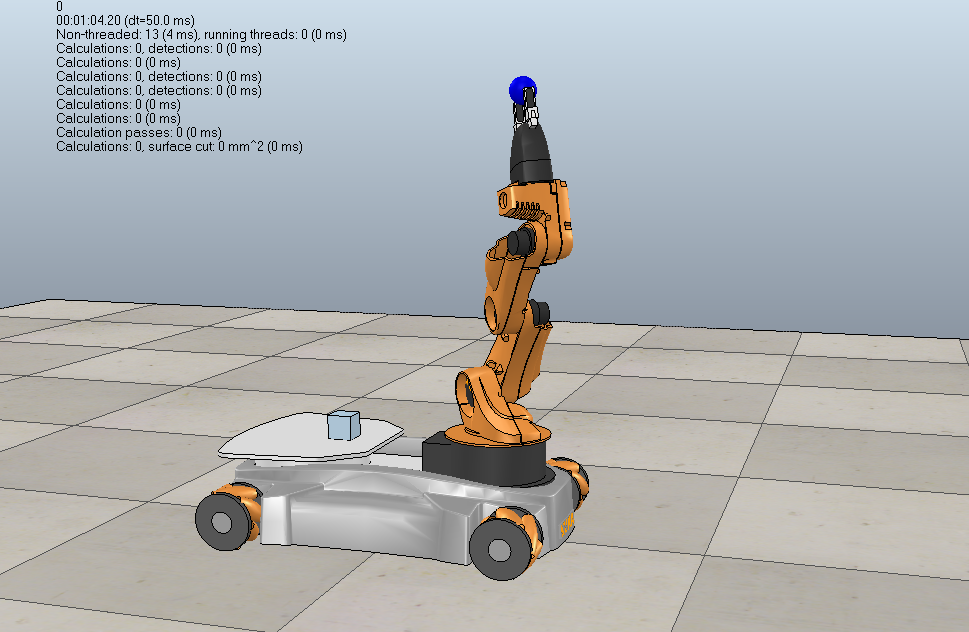
\includegraphics[width=\textwidth]{figures/p2/problem1.png}
    \caption[]%
    {{\small Correct FK calculation}}
    \label{fig:1a}
  \end{subfigure}
  \hfill
  \begin{subfigure}[b]{0.475\textwidth}
    \centering
    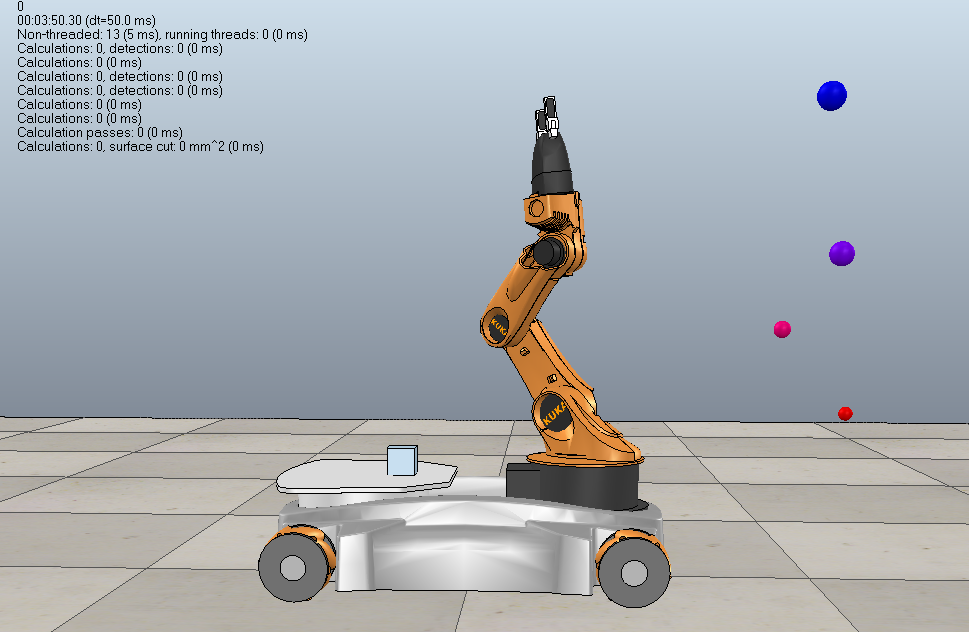
\includegraphics[width=\textwidth]{figures/p2/problem1_debug.png}
    \caption[]%
    {{\small Running in debug mode}}
    \label{fig:1b}
  \end{subfigure}
  \caption{Visualization of forward kinematics calculations. Image (\subref{fig:1a}) shows a correct
    FK calculation with debug mode turned off; note that the blue ball is between the fingers of the
  end-effector. Image (\subref{fig:1b}) shows an example of running the problem in debug mode.}
  \label{fig:1}
\end{figure}

When you run this problem, you will see that the arm moves quickly to a series of random
configurations. If your implementation of the \texttt{fk} service is correct, then you will see a
blue ball between the youBot fingers.

If your implementation has a bug, then it may be difficult to determine from the simulation what is
wrong because the arm moves rapidly. We have therefore provided you with a debug mode. In the file
\texttt{fk.launch}, there is a ROS parameter named \texttt{fk\_debug} that is set to
\texttt{False} by default. When it is set to \texttt{True}, the arm will move slowly through the
entire range of each joint. Furthermore, each ball showing your FK solution will be offset 0.4
meters in front of the robot. If you provide the positions of all five frame origins in the return
value of \texttt{fk}, then using debug mode will help you identify mistakes in your implementation.


\newpage
\appendix

\section{KUKA youBot Design Specification}\label{app:kinematics}

\begin{figure}[h]
  \centering
  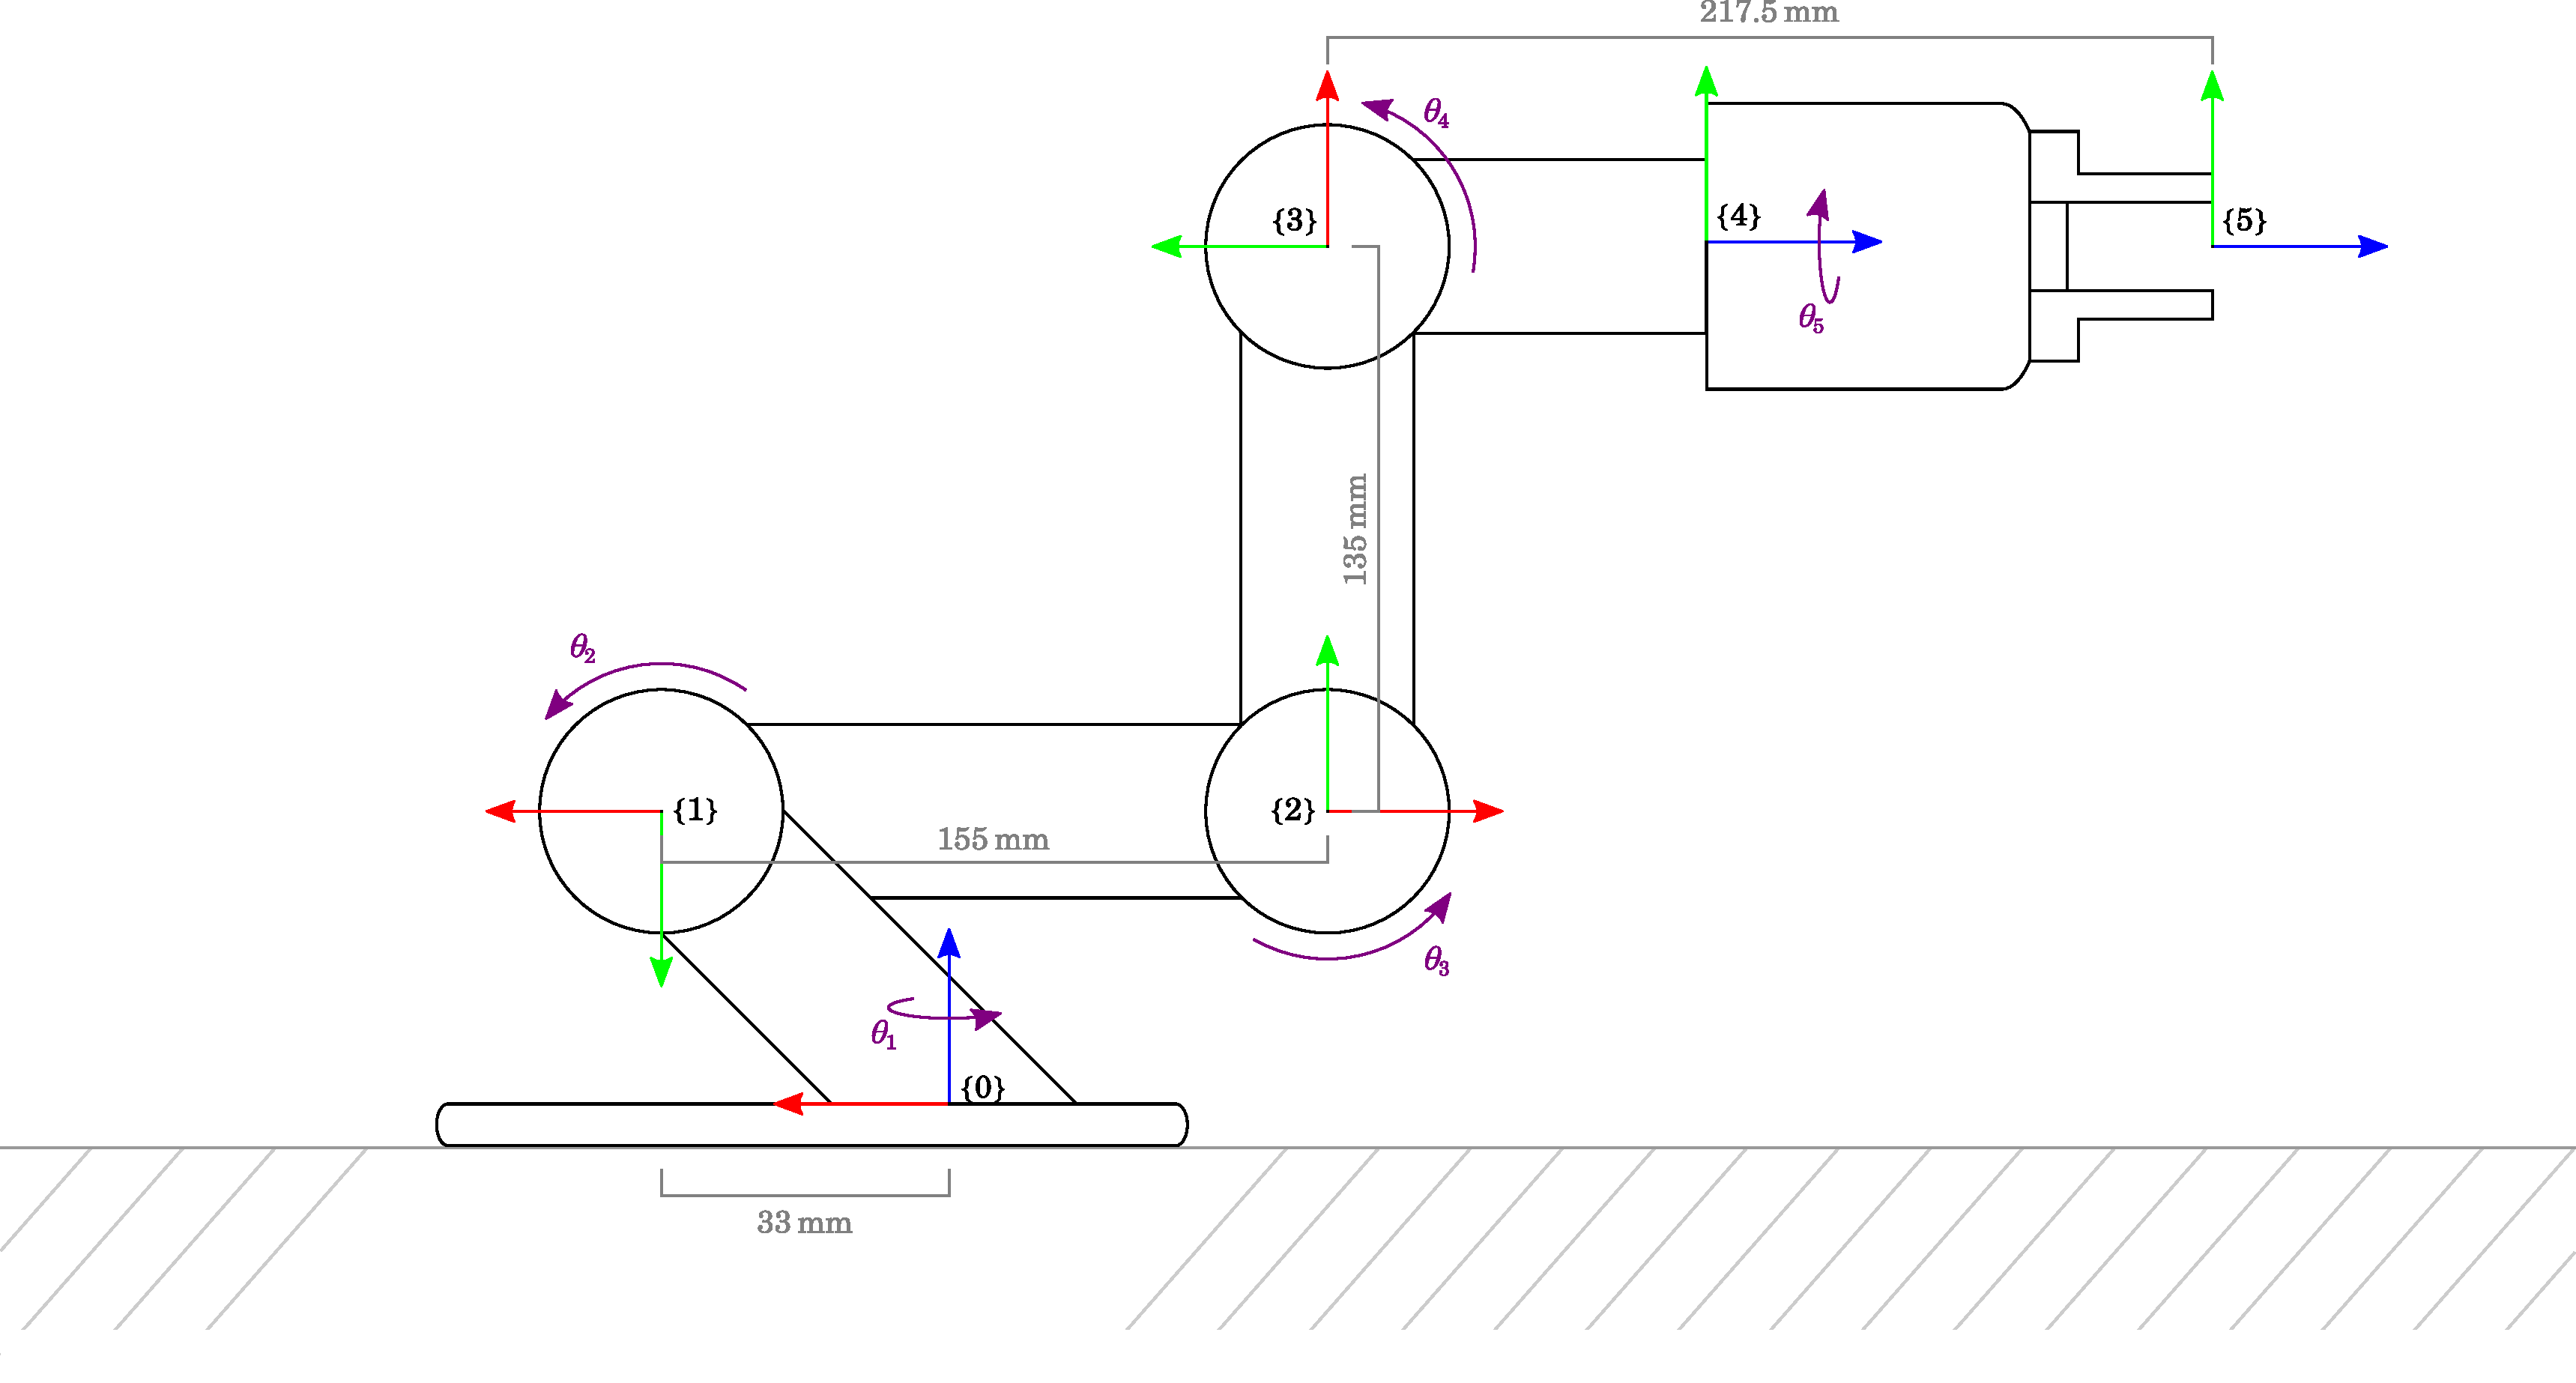
\includegraphics[width=\textwidth]{figures/p2/youBot_specs.pdf}
  \caption{Informal design specification for the KUKA youBot manipulator arm, which has five
    revolute joints and a two-finger gripper. The angle of joint $i$ is given by $\theta_i$, and the
    direction in which the angle is measured is shown with a purple arrow. Each link in the arm has a
    frame rigidly attached to it, and the $x$-, $y$-, and $z$-axes of the frame are shown in red, green,
    and blue, respectively (the one unshown axis for each frame points either out of or into the page).
    Note that $z_i$ is the axis of rotation for joint $i + 1$, \textbf{not} joint $i$. The frames are
    attached in this manner so that when joint $i$ is actuated, link $i$ and its attached frame $\{i\}$
    move. Finally, note that since axes $z_3$ and $z_4$ intersect, the origin of frame $\{4\}$ can be
    placed at any point along $z_4$. We have depicted it at the wrist for the sake of the visual, but in
  practice we would place it at the intersection of $z_3$ and $z_4$ to simplify the math.}
\end{figure}

\newpage

\section{NumPy Overview}\label{app:numpy}

\begin{description}
  \item[Importing NumPy] First, make sure to import NumPy: \texttt{import numpy as np}
  \item[Constructing an array] A NumPy array can be any number of dimensions. To create a
    $n$-dimensional array, you can use \texttt{np.array()}. For example, \texttt{a\_1D =
      np.array([1.,2.,3.])} creates a 1D array of floats, and \texttt{a\_2D =
    np.array([[2,2],[0,1]])} creates a 2D array of ints where the first row is [2, 2] and the second
    row is [0, 1].
  \item[Special arrays] NumPy includes some useful functions to create special arrays. One such
    function is \texttt{np.zeros(shape)}, which returns a $n$-dimensional array of the specified
    shape (a tuple specifying each of the $n$ dimensions). For instance, \texttt{np.zeros((3,2))}
    returns a $3 \times 2$ array of 0s. Another useful function is \texttt{np.identity(n)}, which
    returns a $n \times n$ identity matrix.
  \item[Constructing a matrix] A NumPy matrix is just a special 2D NumPy array. Use
    \texttt{np.matrix()} to create a matrix. For example, \texttt{m = np.matrix([[2,2],[0,1]])}
    creates a matrix with the same values as \texttt{a\_2D} from above. However, while they may be
    very similar and you can do the same things with both, the matrix and array types are not
    exactly the same. Besides the fact that a matrix can only be 2D, an important difference is in
    matrix multiplication, as described next.
  \item[Matrix multiplication] To perform matrix multiplication with the matrix type, you can simply
    use the * operator. For example, we can multiply the matrix \texttt{m} we defined above by doing
    \texttt{m}*\texttt{m}. If you're working with 2D matrices, the matrix type is convenient since
    matrix multiplication is very intuitive. \textbf{Be careful:} In this case, the * operator
    performs matrix multiplication like you might expect. However, if you use $n$-dimensional arrays
    instead of matrices, the * operator will multiply the arrays element-wise. You can do normal
    matrix multiplication with arrays by using NumPy's \texttt{dot()} function. For example,
    \texttt{a\_2D.dot(a\_2D)}, or alternatively \texttt{np.dot(a\_2D,a\_2D)}, will return the same
    matrix product as \texttt{m}*\texttt{m}, and these are NOT equal to
    \texttt{a\_2D}*\texttt{a\_2D}.
  \item[Inverse and transpose] Getting the transpose of a matrix/array with NumPy is easy. You just
    need to use \texttt{.T} (e.g. \texttt{m.T} or \texttt{a\_2D.T}). You can get the inverse of a
    square matrix/2D array using \texttt{np.linalg.inv()}. For example: \texttt{np.linalg.inv(m)}.
  \item[Indexing] You can access specific parts of an array/matrix by indexing particular cells like
    you would expect (e.g. \texttt{m[1,0]} would return 0). You can also use slicing to get subsets
    of a matrix/array. For example, \texttt{m[:,1]} returns the second column of \texttt{m}, where
    the colon selects all of the rows and the 1 specifies the column we want.
\end{description}

For a more in-depth NumPy guide, you can read the quickstart tutorial
\href{https://docs.scipy.org/doc/numpy-dev/user/quickstart.html}{here}.


\end{document}

%%% Local Variables:
%%% mode: latex
%%% TeX-master: t
%%% End:
